%!TEX root = ../../../thesis.tex
\chapter{SMGR}

\section{abstract}

	We introduce the Slime Mold Graph Repository (SMGR), a novel data collection promoting the visibility, accessibility and reuse of experimental data revolving around network-forming slime molds. By making data readily available to researchers across multiple disciplines, the SMGR promotes novel research as well as the reproduction of original results. While SMGR data may take various forms, we stress the importance of graph representations of slime mold networks due to their ease of handling and their large potential for reuse. Data added to the SMGR stands to gain impact beyond initial publications or even beyond its domain of origin. 

	We initiate the SMGR with the comprehensive KIST Europe data set focusing on the slime mold \emph{Physarum polycephalum}. It contains sequences of images documenting growth and network formation of the organism under constant conditions. Suitable image sequences depicting the typical \emph{P.~polycephalum} network structures are used to compute sequences of graphs faithfully capturing them. Given such sequences, node identities are computed, tracking the development of nodes over time. The entire data set is well-documented, self-contained and ready for inspection via the SMGR at \href{http://smgr.mpi-inf.mpg.de}{http://smgr.mpi-inf.mpg.de}.

\section{Introduction}

	Slime molds are interesting and complex organisms providing a rich substrate for interdisciplinary research. One member of the family, \emph{Physarum polycephalum}, has received increasing interest as of late resulting in intensive research efforts that continue to shed light on many aspects of this organism. Of particular interest is its ability to form and maintain complex networks. Efforts to improve our understanding of formation, structure and function of these networks are manifold~\cite{Marwan419,tero2010rules,alim2013random,baumgarten2010plasmodial,baumgarten2013functional} and ongoing.

 	A popular two-step approach, not restricted to slime molds, consists of taking images of the networks formed by the organism and converting them to graphs\footnote{In this context graphs denote abstract mathematical objects, subject of Graph Theory, consisting of vertices and edges. Note that some scientific communities traditionally refer to vertices as nodes or sites and to edges as arcs or links.}. First, images are obtained by cultivating \emph{P.~polycephalum} in the wet-lab whilst documenting the development of the organism and its networks. This is a time consuming process which needs to be repeated sufficiently often under constant conditions to acquire a reliable body of observations. 

 	The second part requires methods capable of analyzing an image and deriving a faithful graph representation of the network depicted therein. Such methods have become available recently as convenient software packages~\cite{dirnberger2015nefi}. Once graphs are available, concepts and methods from Network Science and Graph Theory directly apply, enabling efficient and detailed investigations of graph properties~\cite{baumgarten2012computational,heaton2012analysis}.

 	We stress that both steps are challenging as they require time, special laboratory resources and expert knowledge. Data acquisition and graph extraction in particular, may quickly become serious obstacles deterring interested researchers from starting to work with networks formed by \emph{P.~polycephalum}. 

 	Despite such difficulties, "graph-based" approaches have been quite successful and various interesting results are available today~\cite{baumgarten2010plasmodial,baumgarten2013functional,fessel2014analytical,fessel2012Physarum,ito2011characterization}. However, data used to establish these results, i.e. the graphs and their underlying images themselves, are not nearly as available in many cases. This is unfortunate because due to their ease of handling and their abstraction power, graphs naturally lend themselves to reuse, potentially gaining impact beyond their initial publications or even beyond their domain of origin.

 	Our own experience shows, that most researchers are, at least in principle, willing to share their valuable data. However, data sharing can be cumbersome and constitutes an extra hurdle discouraging data reuse. To combat this, data needs to be collected and made available in an organized fashion. Similar efforts have become best practice for diverse types of data originating in various fields of science. Examples are numerous including collections of images of cells~\cite{cell}, large graphs~\cite{snap} or experimental data in high energy physics~\cite{hepdata}, to name but a few.

	To the best of our knowledge no such repository exists for data concerned with networks of slime molds. For this reason we decided to set up the \emph{Slime Mold Graph Repository} with the goal of providing an available collection of networks focused on slime molds. Although this is clearly a niche topic, we believe that due to the many open question revolving around the structure and function of such networks and their large interdisciplinary appeal, setting up a small but dedicated repository is of value.

	The benefits of such a repository are manifold. Making data available for everyone increases visibility of contributors, allows original results to be reproduced and puts data in a prime position to become a catalyst for novel research. Given the significant costs, i.e. time and resources, which are typically associated with obtaining high quality data, promoting increased reuse of data is an economical choice. Researchers and other professionals that do not have the required resources/connections to produce/obtain their own data sets benefit in particular from repositories like the SMGR, since it provides immediate and convenient access to experimental material that would be hard to acquire by other means. 

	Furthermore, we envision the SMGR to become a mediator between theory and experiment. Theoretical work in biology and biophysics concerned with modeling various aspects of \emph{P.~polycephalum} networks, may utilize experimental data as a testbed for model predictions. This approach has been put into practice previously~\cite{baumgarten2015network}, but was exclusive to researchers in possession of relevant data. With the introduction of the SMGR such limitations are removed. Similar statements can be made for other fields, e.g. Computer Science, which is actively studying \emph{P.~polycephalum} in the context of Natural Computing. Access to experimental data via the SMGR allows to compare theory and experiment and to build the intuition crucial to theoretical investigations and modeling efforts. 

 	In order for the SMGR to be useful from day one, we initiate the repository with our own extensive data sets obtained at the \emph{KIST Europe}. It is important to us, that anyone can go the SMGR project page, download any available data and immediately start working with it in whichever way he or she chooses. The data set we provide also serves as a possible example for the type of data the SMGR intends to collect and what level of documentation is appreciated. 

 	We stress at this point that the SMGR is not intended to be a simple archive to permanently store data. First and foremost, we seek to collect data that has not yet been fully explored or has a strong potential to be of use to others. The KIST Europe dataset fulfills both criteria.

 	In the following we discuss the concept of the SMGR and give a detailed account of the contents of the KIST Europe data set and how it was obtained. We also provide suggestions for further use of the KIST Europe data.

\section{Repository concept}
	
	Today the impact of data sharing as a scientific practice is ever increasing. Currently, two major forms of data collections are commonly encountered.

	First, data is collected in large, well-organized repositories holding enormous amounts of information. Such major repositories easily contain thousands of datasets, covering numerous topics across its domain of relevance. Due to their size and complexity, curating and maintaining such repositories requires major resources typically provided by larger research institutions or non-profit organizations. 

	Most major data collections, however, have started as small and specialized repositories at some point. Such repositories constitute the second approach to data sharing common today. These are typically much simpler in structure and contain a smaller number of datasets. Small repositories tend to be more specialized and have very close ties to their relevant research communities since the operators of the repository are often researchers themselves. Smaller repositories can operate with minimal infrastructure requirements since changes to the repository are less frequent and data sets are limited in number and size.

	With the SMGR we seek to establish a collection of research-grade data revolving around network-forming slime molds. Given the highly specialized nature of the topic, we believe that setting up a small stand-alone repository is the correct choice to begin with. A small repository is very flexible and can adapt and evolve more easily based on community feedback. In this form the idea of the SMGR was first introduced at PhysNet 2015 and was well received with individuals signaling their willingness to contribute data~\cite{physnet2015}. We strongly believe that a tight integration with the research community, is key to the future success of the SMGR. 

	Any repository needs a set of instructions, policies and requirements applying to data submission, data usage and various other general aspects of repository operation. For these the SMGR relies on established best practices of data sharing whilst striving to keep things as straight-forward as possible~\cite{white2013nine}. A detailed account can be found on the \href{http://smgr.mpi-inf.mpg.de}{SMGR project page}, which we consider the main part of this contribution. We opt to treat policies, user instructions and other important questions in a comprehensive FAQ on the \href{http://smgr.mpi-inf.mpg.de}{SMGR project page} rather than in this manuscript, simply because they are subject to future change.

	The SMGR and all available data can be found here: \href{http://smgr.mpi-inf.mpg.de}{http://smgr.mpi-inf.mpg.de}.



\section{The KIST Europe data set}	

	In order to make the SMGR useful from day one, we initiate the repository with a comprehensive data set revolving around networks formed by \emph{P.~polycephalum}~\cite{lifecycle}. 
	In the following we present a short description of the KIST Europe data set designed to give the interested reader a high-level understanding of its nature and content. In addition, we recommend to inspect the data directly using the browsing and download functions provided on the \href{http://smgr.mpi-inf.mpg.de}{SMGR project page}. We refer the expert reader, interested in reproducing all the steps involved in the creation of the data set, to an in-depth exposition given in the Materials and Methods section.

	The KIST Europe data set contains raw and processed data obtained and derived from $81$ identical wet-lab experiments, carefully executed under constant conditions. Figure~\ref{fig:setup} illustrates the experimental setup used. The data was produced using the following procedure:

	\begin{enumerate}
		\item A rectangular plastic dish is prepared with a thin sheet of agar.
		\item A fixed amount of dried \emph{P.~polycephalum} (HU195xHU200) sclerotia crumbs is lined up along the short edge of the dish, see \Fref{fig:sequence_1}. The dish is put into a large light-proof box.
		\item After approximately $14$ hours the plasmodium resuscitates and starts exploring the available space towards the far side of the dish. Typically, the apical zone needs to cover a distance of several centimeters before network formation can be observed properly, see \Fref{fig:sequence_2}.
		\item For the next $30$ hours we take a top-view image of the growing plasmodium and the changing network every $120$ seconds from a fixed position. A typical obtained image is seen in \Fref{fig:sequence_3}. We stop capturing when the apical zone is about to reach the far side of the dish, which is well outside of the observed area. 
		\item After obtaining sequences of images showing the characteristic networks of \emph{P.~polycephalum}, we use a software called NEFI to compute corresponding sequences of graph representations of the depicted structures within a predefined region of interest~\cite{dirnberger2015nefi}, see \Fref{fig:sequence_4}. The graphs store precise information of the length and width of the edges as well as the coordinates of the nodes in the plane. A typical resulting unfiltered graph is seen in \Fref{fig:sequence_5}.
		\item Given the resulting sequence of graphs we apply filters removing artifacts and other unwanted features of the graphs. Then we proceed to compute a novel node tracking which encodes the time development of every node taking into account the changing topology of the evolving graphs.
	\end{enumerate}

	\begin{figure}
		\centering
		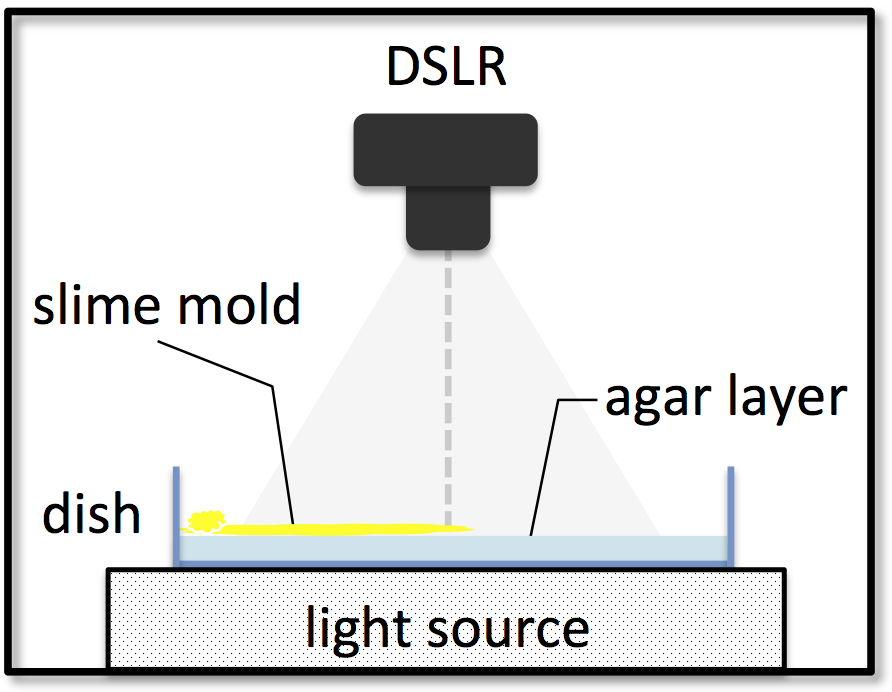
\includegraphics[width=\linewidth,keepaspectratio]{setup.png}
		\caption[Setup for wetlab experiments.]{Schematic description of the experimental setup.}
		\label{fig:setup}
	\end{figure}

	\begin{figure}
		\centering
		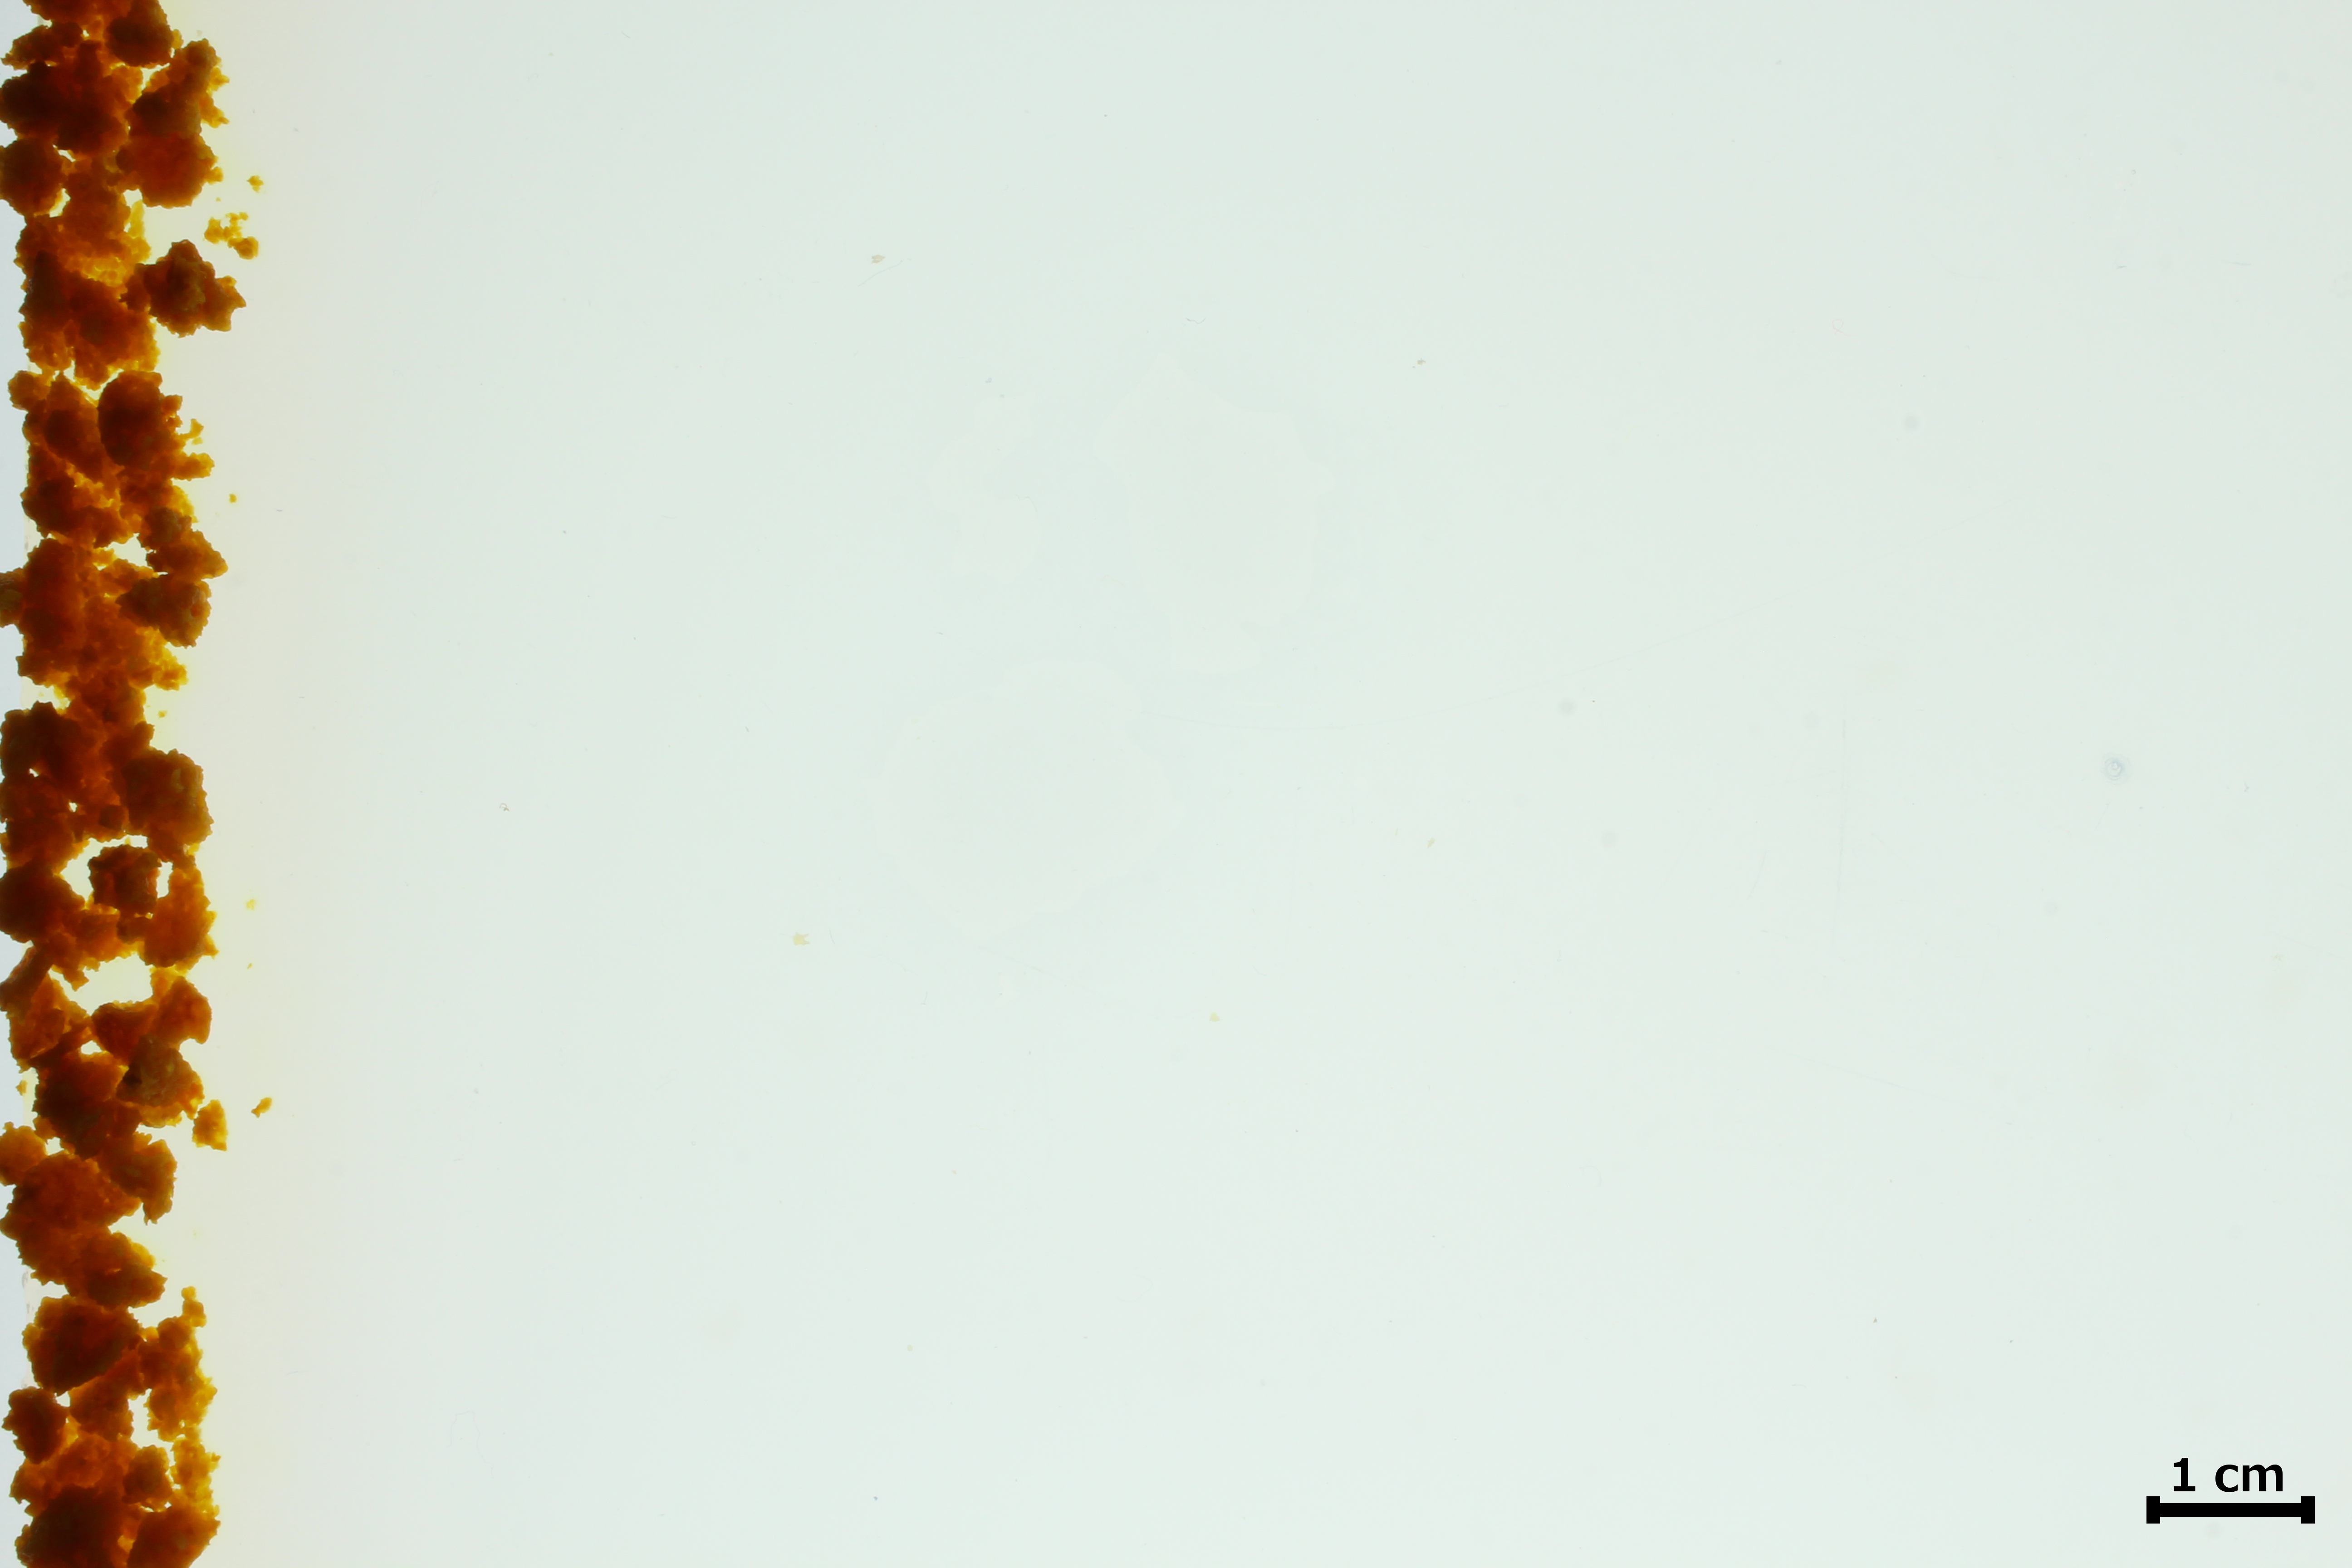
\includegraphics[width=\linewidth,keepaspectratio]{physarum_sequence_1.JPG}
		\caption[Crumbs of \P sclerotia forming an inoculation line.]{Crumbs of \P sclerotia forming the inoculation line.}
		\label{fig:sequence_1}
	\end{figure}

	\begin{figure}
		\centering
		\includegraphics[width=\linewidth,keepaspectratio]{physarum_sequence_2.JPG}
		\caption[The apical zone advances.]{The plasmodium explores the dish. The apical zone advances towards the right side of the dish supported by a complex network that is continuously forming.}
		\label{fig:sequence_2}
	\end{figure}

	\begin{figure}
		\centering
		\includegraphics[width=\linewidth,keepaspectratio]{physarum_sequence_3.JPG}
		\caption[The onset of network coarsening.]{As the apical zone is about to escape the observation region, the coarsening of the network becomes more pronounced.}
		\label{fig:sequence_3}
	\end{figure}

	\begin{figure}
		\centering
		\includegraphics[width=\linewidth,keepaspectratio]{physarum_sequence_4.JPG}
		\caption[A complex network of veins within a region of interest.]{The apical zone has moved on, leaving behind a complex network of veins. The dashed rectangle depicts a typical region of interest relevant for subsequent image analysis and graph detection.}
		\label{fig:sequence_4}
	\end{figure}

	\begin{figure}
		\centering
		\includegraphics[width=\linewidth,keepaspectratio]{physarum_sequence_5.JPG}
		\caption[Graph extracted from the sample region of interest.]{The network within the region of interest has been extracted by NEFI. Note that no filters have been applied. Dead ends and nodes of degree 2 are visible still, leading to small patches of nodes appearing to clump up. Such artifacts can be removed in suitable post-processing steps.}
		\label{fig:sequence_5}
	\end{figure}

	Repeating this experiment we obtain $81$ similar sequence of images, which we consider our raw data. We stress at this point that given the inherently uncontrollable growth process of \emph{P.~polycephalum}, the obtained sequences differ in length and nature. In some experiments the organism behaved unfavorably, simply stopping its growth, changing direction or even escaping the container. While such sequences are part of the raw dataset, we excluded them partially or completely from the subsequent graph extraction efforts. The removal of such data reduces the number of series depicting optimal network formation to $54$.

	After obtaining the raw data, we transform the images into equivalent mathematical graphs, thus opening up a wealth of possibilities for data analysis. To this end we deploy a convenient automatic software tool called NEFI~\cite{dirnberger2015nefi}, which analyzes a digital image, separates the depicted slime mold network from the background and returns its graph representation. Using this tool effectively requires moderate amounts of image preprocessing. In particular, for each sequence of images it is necessary to decide on a suitable subsequence to be processed. Here we typically exclude parts of the sequence where the apical zone is still visible. For each such subsequence a suitable region of interest is defined manually. \Fref{fig:sequence_4} depicts a typical choice for the region of interest to be processed by NEFI. The established unfiltered graph can be seen in \Fref{fig:sequence_5}. The graph stores the position of the nodes in the plane as well as edge attributes such as edge length and widths for each edge. In addition to the output of NEFI including the unfiltered graphs, the dataset contains NEFI's input, i.e. the selected subsequences of images cropped according to their defined regions of interest.

	Note that some parts of the image series showing proper network formation did not yield optimal representations of the depicted networks. This is a result of images exhibiting strong color gradients or other effects rendering them too challenging for automatic network extraction. While such cases may still be handled by tuning the parameters of image processing manually on an image per image basis, we decided to discard affected series from subsequent processing efforts. As a result the number of usable graph sequences of highest quality reduced to $36$. To this we apply a set of filters removing artifacts, isolated small components and dead-end paths. Thus we obtain a total of $3134$ distinct filtered graphs faithfully reflecting the topology and edge attributes that \emph{P.~polycephalum} displayed during the wet-lab experiments. At this point available graph analysis packages or custom written analysis code can be deployed to investigate the data in various ways, e.g.~\cite{ICWSM09154,schult2008exploring}. The dataset includes the filtered graphs as well as all corresponding graph drawings. The latter enable a quick visual inspection of the graph extraction results.

	Given the obtained time-ordered sequences of graphs the development of the entire graph can be investigated. One may also study what happens to single nodes as \emph{P.~polycephalum} evolves. Given a graph in a sequence of graphs, let us pick any node $u$. Can we determine a set of nodes from graphs in the sequence that are equivalent to $u$, i.e. all nodes in the set are earlier or later versions of $u$ in time? We answer this question by computing a so-called \emph{node tracking} which establishes the time development of all nodes in the graph. Crucially, this tracking takes into account topological changes in the evolving graphs. The result of the tracking is available as node properties of the graphs. Naturally, the program computing the tracking is included in the dataset. To the best of our knowledge, this type of data is made available for the first time through the KIST data set.

	Finally, in addition to the actual data, i.e. images and graphs, the KIST Europe data set contains scripts and larger programs used to process and evaluate the data. Suitable configuration files specify the used regions of interest and the parameters used with NEFI. Thus it is possible to repeat the entire data production process from the raw images to the obtained filtered graphs including the tracking of nodes. As part of the SMGR, the KIST Europe data set is well-structured and self-contained. In particular, sufficient on-the-fly documentation is available when using the online browsing function of the SMGR.

	\subsection{Suggested usage of the KIST Europe set}

		Previously, the data contained in the KIST Europe set has been the subject of initial analysis by the authors of this manuscript~\cite{dirnberger2016}. When exploring time series of \emph{P.~polycephalum} graphs, a particular focus was placed on edge properties, the structure of faces, cuts and percolation properties. In the process, additional questions regarding the nature of \emph{P.~polycephalum} graphs naturally arose. In particular, one may determine whether there is a similarity between \emph{P.~polycephalum} networks and Voronoi graphs. The latter are well-studied and it is interesting to explore a possible connection between their properties and the features of \emph{P.~polycephalum}. A different suggestion consists of answering the question whether \emph{P.~polycephalum} graphs are geometric spanners. Spanners have properties that enable efficient communication between different parts of the graph, a feature clearly relevant and desirable for an organism such as \emph{P.~polycephalum}. Lastly, at the time of writing this manuscript the novel information provided by the computed node trackings is yet to be used for the first time. What can be inferred from the topological changes recorded? Can one identify patterns with certain structural properties? Can topological properties be related to questions of biological relevance? Given the large number of graphs in the SMGR, an investigation of such questions becomes a viable option.
		
		Admittedly, most of the suggestions given so far are inspired by our own interdisciplinary research interests. However, future investigations are hardly limited to them alone. It is fair to say that any observable defined on a weighted graph, relevant to \emph{P.~polycephalum}, can be studied using the KIST Europe set. In particular, we'd like to stress the implications for evaluating and guiding all sorts of theoretical modeling approaches based on graphs. Any model that produces a prediction which can be formulated as an observable defined on a graph can immediately be tested on the KIST Europe set. This includes time dependent observables. Predictions that agree with the SMGR data may increase the trust in a given model, while discrepancies between predictions and data hopefully suggest improvements. Thus, data contained in the KIST Europe set may be used to drive modeling efforts and help bridge the gap between theory and experiment.

		Finally, we like to stress that the KIST Europe constitutes a flexible basis to work with since it contains a host of useful data, code and instructions. In particular, potential users are not limited to working with the graphs that are presently provided. They are encouraged to start from the raw images and determine their own specific data selection and graph extraction procedures tailored to their particular research agenda. They may use the tools provided by us or deploy entirely different strategies to better suit their needs.

	\subsection{Materials and methods}

	    In this section we explain all steps involved in furnishing the KIST Europe dataset in full detail. First, we describe how to setup and execute necessary wet-lab experiments, including the production of sclerotia~\cite{lifecycle}. Next, we explain how to turn the network structures depicted in the raw images into series of equivalent graphs. Finally, we illustrate how to establish unique node identities and track them within a given series of graphs.

	    \subsubsection{Obtaining experimental data}

	      For our experiments we cultivate \emph{P.~polycephalum} (HU195xHU200) in a rectangular, $20$~cm $\times$ $30$~cm $\times$ $13$~cm, translucent plastic dish ontop of a $10$ mm layer of $1.25 \ \%$ agar (Kobe I). To do so we place $1.5$ g of dried \emph{P.~polycephalum} sclerotia crumbs along the short edge of the dish. We make sure to evenly spread them out such that a continuous and straight line is formed, connecting two adjacent edges of the dish. In the following we refer to this line as the \emph{inoculation line}, see \Fref{fig:sequence_1}. This concludes the preparation of the dish. 

	      Since \emph{P.~polycephalum} is sensitive to light, we place the dish inside a large light-proof wooden box of $110$~cm x $110$~cm $110$~cm. Temperature and humidity inside were kept constant at \SI{22}{\celsius} and $55-60 \ \%$ relative humidity. In our setup we rely on dried sclerotia, rather than plasmodium, because the former give exact control over the initial mass of \emph{P.~polycephalum} introduced to the dish. We make sure to keep the input masses, the properties of the agar layers and the environment constant to ensure consistent repetition of experiments. For a detailed description on how to produce dried sclerotia from an initial sample we refer the reader to the supplementary material.

	      Inside the box we fix a digital camera (Canon EOS 645D, Lens EFS 18-55 mm) $16$~cm above the dish. The camera is oriented perpendicular to the dish and centered right above it. Each shot captures a large area of $10$~cm $\times$ $15$~cm at a resolution of $5184 \times 3456$ pixel in JPG format. With these settings $1$~cm on the dish corresponds to $370.625$~pixels in the image. Since during graph extraction all lengths and widths measured are stored in units of pixel, this information can be used to map pixels back to centimeters.

	      To provide the necessary light for the camera to work inside the dark box we opt for bright field illumination using a negatoscope, also known as X-ray film viewer (Planilux, $2 \times 15$ W, emitting white light). It provides a large area of low intensity illumination which is uniform in space and time. By putting the translucent dish ontop of the negatoscope the light that passes trough makes the structures formed by \emph{P.~polycephalum} visible to the camera overhead. By design we ensure optimal contrast between the networks and the background and eliminate all sources of reflections or shadows in the images. This is particularly desirable as such effects are diminishing the effectiveness of the software used to do the graph extraction. This concludes the preparation of the box. A schematic of the complete setup can be seen in \Fref{fig:setup}.

	      After the prepared dish is placed in the box, it takes roughly $15$~hours for the organism to make its transition from sclerotia to plasmodium. Once the plasmodium begins to spread towards the far side of the dish we start capturing its growth progress by taking an image every $120$~seconds using dedicated software (Motion detection software; Vulpessoft, DSLR Master). We stop capturing when the growing front first hits the adjacent wall of the dish. By doing so we minimize the probability of \emph{P.~polycephalum} moving back towards the inoculation line. We do not feed the organism throughout the entire experiment. This concludes one iteration of our experiments.

	      We repeat this experiment under constant conditions and obtain $81$~image series depicting the growth of \emph{P.~polycephalum} and the networks it forms. Since there is a natural variability in the growth of the organism, we obtain series of different length and nature. We refer to this data as raw data.

	      We are aware of a potential caveat of our approach, namely the light source in the negatoscope emitting the full spectrum of white light. It is well known that \emph{P.~polycephalum} reacts to specific parts of the spectrum while it is insensitive to others~\cite{nakagaki1996action}. Thus, ideally one chooses a light source such that the organism remains undisturbed. However, such a light source was not at our disposal so we decided to minimize the impact of the light by minimizing the time \emph{P.~polycephalum} is exposed to it. In particular we couple the triggering of the camera with the power supply of the negatoscope. Thus we ensure that the slime mold is illuminated a mere $1$~second every $120$~seconds. Since we did not observe any irregularities in our experiments known to be induced by light we conclude that our precautions were sufficient.

	    \subsubsection{Graph extraction}

	      Given the obtained raw data, we discard all series that do not show proper network formation. Thus the number of usable datasets is reduced to $54$. For the remaining series we seek to describe the characteristic \emph{P.~polycephalum} networks by equivalent graphs. In addition to capturing the topology of the networks, we want to obtain a precise measure on the length and width of each vein observed. Furthermore, we want to establish the positions of the junctions of the veins in the image. Thus, we want to compute a weighted graph, whose nodes carry the positions of the junctions in the plane and whose edges carry weights corresponding to the length and the width of the observed veins. 

	      To compute such a graph representation we rely on a software tool called NEFI. This tool takes as input an image from the raw dataset depicting a network and returns a faithful representation of this network in form of a weighted undirected graph. NEFI offers several different algorithms and a variety of settings to do graph extraction. Some experimentation was necessary to find a sequence of algorithms, a so-called pipeline, such that the returned graph representations preserve as much information as possible. The pipeline has been stored and is part of the dataset for reasons of reproducibility. Asserting the effectiveness of a pipeline is convenient and easy, since the tool allows to visually compare the computed graph with the network in the input image by drawing the former ontop of the latter. An example can be seen in \Fref{fig:sequence_5}. For a more detailed discussion of the reliability of NEFI and how to use it, we refer to its \href{http://nefi.mpi-inf.mpg.de}{project page} and companion paper~\cite{dirnberger2015nefi}.

	      The main caveat of NEFI is that, like any form of image processing or computer vision, the quality of the output strongly depends on the quality of the input. To obtain good results with this tool, the input image must be of high contrast and void of strong color gradients and other detrimental effects~\cite{dirnberger2015nefi}. Due to the design of our experiments these requirements are largely satisfied. However, due to its implementation NEFI struggles with parts of the image that do not depict networks. In particular it fails to process regions depicting the inoculation line and the apical zone. For the network extraction to succeed these areas must be removed from the images or equivalently a region of interest must be defined excluding such areas. For consistency we define a specific region of interest for each given image series of the raw data set. A typical region of interest is seen in \Fref{fig:sequence_4}.

	      To do so, we visually inspected every single image of every sequence in order to decide on a maximal region of interest containing properly formed networks. It is common that somewhere within an image sequence \emph{P.~polycephalum} starts to deviate from "well-behaved" growth, effectively disqualifying the sequence from this point on. Examples include \emph{P.~polycephalum} suddenly reversing direction or spontaneously spawning new growing tips within an already established network. Thus we make two choices: First, for each sequence of images we find the longest usable subsequence and second, for each subsequence we decide on one region of interest. We store this information in small configuration files suitable for automated graph extraction. We point out that in general it has been beneficial if the choices of selection are made somewhat defensively, leading to a reduced likelihood of artifacts occurring in the graph detection process.  

	      Given the configuration files and the extraction pipeline, NEFI can be used to batch process sequences automatically. Note that for some series, partially containing strong color gradients in the background, NEFI failed to properly segment the input images resulting in unusable graphs. This situation can be detected easily by inspection of the segmented images or the graph drawings produced by NEFI. The affected series and the resulting graphs are then excluded from further processing. While this reduces the number of usable graph series to $36$, the remaining graphs capture the topology of the original \emph{P.~polycephalum} networks exceptionally well. 

	      Note that the raw graphs obtained so far are likely to contain artifacts such as isolated nodes and dead-ends, see \Fref{fig:sequence_5}. This is to be expected since NEFI cannot reliably resolve structures that are very fine grained, e.g. veins in the network with a width of less than $5$~pixel. As a result small structures in the graph break up into several disconnected parts. In a similar fashion spurious isolated nodes can enter the computed graph. We strongly recommend anyone considering to work with the raw graphs to carefully inspect them first in order to assess whether these artifacts need to be removed using filters. In our experience, a moderate amount of filtering is always appropriate and considerably improves quality of the graphs, i.e. the degree to which they resemble the original \emph{P.~polycephalum} networks.

	      To deal with the mentioned artifacts NEFI comes with the possibility to apply filters capable of removing isolated nodes and dead ends. We have filtered all raw graphs to obtain the final set of graphs which we store in several file formats. In particular we removed all edges that are not on a cycle, i.e. dead ends are removed, and kept only the largest connected component. For all but the finest of veins the filtered graphs capture the structure of the original \emph{P.~polycephalum} networks extremely well. Furthermore they carry precise information about node positions, edge widths and edge lengths. For a detailed description of how to work with the actual graph files produced by NEFI we refer to its \href{http://nefi.mpi-inf.mpg.de}{project page}.

	      Lastly, we point out that the process of graph extraction described here is geared towards answering a particular set of research questions, see~\cite{dirnberger2016}. For a different set of questions changes may be appropriate and necessary. They can easily be implemented by starting with the raw graphs and applying different filters. Also, it is not difficult to go back even further to the original image sequences and select different regions of interest and different subsequences, leading to different series of raw graphs. Given NEFI and the possibility to use configuration files to automate the graph extraction, it becomes possible to adapt the data in the KIST Europe set to various particular needs.

	    \subsubsection{Node tracking}

	      In this section we explain how to compute a node tracking. Our approach is a variant of a tracking method introduced previously~\cite{woll2013novel,Karrenbauer2013}. Here we give a self-contained account of the tracking technique geared towards non-experts in optimization. For technical details, proofs and an experimental evaluation of the method we refer the interested reader to the original publications.

	      For each of our experiments, let us denote the respective time ordered sequence of $k$ filtered graphs with $\mathcal{G} = {G_1, G_2, \dots, G_t, \dots, G_k}$ and the union of the respective node sets with $\bar{V} = \bigcup_{i=1}^{k} V_{k}$. Each node in $\bar{V}$ can be represented as a non-negative integer triple $(x,y,t)$. Here $x$ and $y$ denote a node's pixel coordinates relating to the input image used for graph extraction and $t$ denotes its position in the sequence, i.e. in time.

	      We seek to exploit this information to partition the set $\bar{V}$ into a collection of disjoint, time-ordered paths such that every $u \in \bar{V}$ is part of exactly one path. We call such a path a \emph{track} and assign an unique identifier to it, e.g. a unique color, which is shared by all nodes in the track. Intuitively speaking, rather than thinking of a track as a collection of nodes, one can interpret it as one physical node observed at different points in time.

	      Let us define the length of a track by the number of nodes it contains. We stress that in general a track need not have length $k$. Tracks may start at any $t=i$ such that $1 \le i \le k$ and end at any $t=j$ such that $i \le j \le k$. In particular tracks of length $1$ are possible. Crucially, any node in a track has at most one predecessor and at most one successor node.

	      Let us refer to the edges within a track as \emph{tracking edges}. Tracking edges may connect nodes of temporal distance larger than $1$, i.e. $e = (u,v) = ((x_u,y_u,t_u), (x_u,y_u,t_v))$, where $1 \le t_u < t_v \le k$. Such tracks simply "skip" nodes between the start and the endpoint of the track and correspond to nodes that have not been observed by NEFI for some amount of time. Given the continued changes in the network topology observed during the growth of \emph{P.~polycephalum} such tracks are expected to appear frequently. 

	      Let us elaborate on two effects that impact said topology. First, \emph{P.~polycephalum} networks tend to coarsen as time goes by. Eventually, this process may cause the thickness of receding veins to slowly drop below the detection threshold of NEFI. Hence, they disappear from the graphs leading to tracks of length much shorter than $k$. Second, periodic changes in the thickness of veins are observed. It may happen that the thickness of a subset of contracting veins may drop below the detection threshold of NEFI. As a result, those veins disappear from the graph. However, as the contraction cycle of the vein proceeds its thickness may increase again, eventually exceeding the detection threshold and thereby returning to the graph. These periodic changes in the topology of the graphs naturally lead to tracks that skip a certain number of frames periodically. Both effects are present at the same time and can be observed in the graphs we have obtained.

	      We stress at this point that given a time resolution of $120$~seconds, one must not use the graphs contained in the KIST data set to study the sinusoidal behavior of edge thickness due to peristaltic pumping. The period of pumping is known to be approximately $100$~seconds and can thus not be properly resolved~\cite{stewart1959protoplasmic}. However, changes in topology are on a much slower time scale and are reliably reflected by the graphs.

	      We proceed to explain how to compute a node tracking. Let us study the graph in \Fref{fig:tracking} to gain some insight into the problem. Consider e.g. node $a_1$. We seek to find a unique track that contains this node, representing its development in time. A straight-forward suggestion would be a track $T_a = [a_1,a_2,a_3]$. However the track $T_a = [a_1,c_2,f_3]$ is just as valid, as is $T_a = [a_3]$ and so forth. The example illustrates that the number of possible tracks and therefore the number of disjoint partitions into tracks grows exponentially with the number of nodes involved. 


	      \begin{figure}
	        \includestandalone[width=.3\textwidth]{tracking/tracking_1}
	        \includestandalone[width=.3\textwidth]{tracking/tracking_2}
	        \includestandalone[width=.3\textwidth]{tracking/tracking_3}
	        \caption[Schematic description of node tracking.]{Schematic of a graph and its changing topology with respect to time. At time $t=2$ the edge $(b,e)$ and its nodes disappear from the graph because the thickness of the corresponding vein in \emph{P.~polycephalum} dropped below the detection threshold of NEFI. The colors indicate tracks $T_b$ and $T_e$ for nodes $b$ and $e$ respectively.}
	        \label{fig:tracking}
	      \end{figure}

	      Ultimately, we seek to find a partition, that faithfully captures the time development of the nodes in $\bar{V}$. To do so we rely on the observation that optimal tracks are likely to consist of nodes that are close in space as well as close in time. In the following we formalize this requirement and construct a linear program (LP) that selects an optimal partition amongst all possible partitions. Once an LP has been defined, solving it becomes a standard task of optimization and can be done efficiently using solvers like Gurobi~\cite{optimization2012gurobi} or Cplex~\cite{cplex2005high}.

	     Let us define the optimization problem we want to solve. First, we construct all possible tracking edges using space partition techniques. Assigning a unique identifier to each edge we obtain the set $\bar{E}$. When the linear program considers edges to include in a possible tracking solution it refers to them using the ids in this set. We define the cost of selecting a particular tracking edge $e = (u,v) = ((x_u,y_u,t_u), (x_v,y_v,t_v))$ as
	      
	      \begin{equation}
	        \Delta(e) = \epsilon ((x_u - x_v)^2 + (y_u - y_v)^2 ) + \tau (t_u - t_v)^2,
	      \end{equation}
	      where $\epsilon$ and $\tau$ are constants used to control the relative strength of the squared Euclidean distance in space and time respectively. Note that using this cost function in our example in \Fref{fig:tracking}, track $T_a = [a_1,a_2,a_3]$ is favored over $T_a = [a_1,c_2,f_3]$. Note also that tracks of length $1$ have cost $0$ since there are no tracking edges to pay for. As a result the minimum cost solution consists of singleton tracks and is not very useful. To circumvent this problem we assign dedicated costs to any node that starts or ends a track as

	      \begin{equation}
	        p(u) = C.
	      \end{equation}

	      Here it is important that $C$ is selected carefully. It must not be too small since this will force the formation of artificial singleton tracks even if these are not part of the ground truth. Too large a value may artificially suppress singleton tracks which may be part of the ground truth. Going back to Figure~\ref{fig:tracking}, assuming $\epsilon = \tau = 1$, a choice of $ 1 < C < 2^2 = 4$ will lead to two singleton tracks for the node $b$, namely ${b_1}$ and ${b_3}$ because a tracking edge connecting $b_1$ and $b_3$ comes at an edge cost of $\Delta(e)=4$. Increasing the node cost such that $C>2^2 = 4$ changes the picture and results in the desired tracks $T_b = [b_1, b_3]$ and $T_e = [e_1, e_3]$. The example illustrates the importance of the constants involved in the cost functions.

	      Note that, we are still facing an exponential number of tracks to consider. Luckily, we can reduce the size of the set $\bar{E}$, and thus the size of the LP, dramatically by combining the effect of the costs functions with additional assumptions that valid for tracking \emph{P.~polycephalum} graphs. In particular, the cost functions imply that we favor non-singleton tracks with nodes that are close in time as well as space. As a result, we may discard all options that have a geographical distance larger than a certain $R$ and a temporal distance larger than a certain $T$. Intuitively, when trying to find all possible tracking edges for a node $u$, we likely need not consider nodes that are located on the other side of the graph or have an unrealistically large temporal separation. Instead we can restrict the search to tracking edges within a cylinder centered at $u$ with radius $R$ and a height of $T$. We can exclude all tracking edges outside such a search cylinder, because their resulting costs are such that the linear program will never select any of them. 

	      The problem thus boils down to determining suitable values for $R$ and $T$. Since the nodes of \emph{P.~polycephalum} are well-separated and do not move within a time period of $120$~seconds, a small radius of $R = 30$ pixels is justified. We choose $T = 10$ which amounts to a time period of $1200$~seconds to look for tracking edges in temporal direction. To tie the cost of singleton tracks to the physical features of our experiment, we choose $ C = 2 R^2 + T^4$. Setting $\epsilon =1$ and $\tau = 10$ completes the set of constants involved in the tracking problem. With these choices we follow the approach in~\cite{Karrenbauer2013}.

	      We convinced ourselves that these settings are suitable for dealing with \emph{P.~polycephalum} graphs by computing node trackings on artificial test graphs which enable a comparison with known ground truths. To obtain one such series we take a real \emph{P.~polycephalum} graph and randomly remove a certain fraction of nodes from it to obtain artificial graphs at later times. Furthermore we slightly perturb the coordinates of all the nodes of these graphs. As expected we find the error rate to strongly depend on the strength of the geographical perturbation of nodes. As long as the perturbation is smaller than the minimum distance between nodes, the computed tracking is identical to the ground truth. When nodes start moving more from frame to frame, there is a danger that they randomly move past each other. As a result they end up swapping their respective tracks introducing an error. When the perturbation is set such that a node can only move within a radius of $R=30$, less than $4\%$ of the nodes end up in wrong tracks given the settings illustrated above. However, we expect that this error is somewhat pessimistic because nodes in real \emph{P.~polycephalum} do not move much compared to our artificial test graphs. Careful visual inspection of the obtained node trackings resulting from real \emph{P.~polycephalum} data supports this conjecture.

	      From the arguments in the previous section it also follows that filtering has a strong impact on the quality of the node tracking. If graphs are filtered such that nodes are well-separated, excellent results can be expected. Thus, we recommend to carefully apply filters if any research questions based on the node tracking are to be tackled. In particular, contracting nodes of degree 2 is strongly advised.

	      Finally, by combining the considerations discussed above, we are in a position to define the actual linear program computing a node tracking:

	      \begin{alignat*}{4}
	        minimize & : & \ \ f = &\sum_{ e \in \bar{E} } \Delta(e) x_{e}  &+  \sum_{ i \in \bar{V}} p(i) y_{i} & +   \sum_{ \substack{j \in \bar{V}}} p(j) z_{j} &  
	      \end{alignat*}

	      \begin{alignat*}{3}
	          s.t.:
	                & \ \     & \forall \ e \in \bar{E} : \ x_{e} \ge 0  \quad \quad    & \forall \ i \in \bar{V} : \ y_{i} \ge 0                                          & \forall \ j \in \bar{V} : \ z_{j} \ge 0                                             \\
	                & \ \     & \forall \ i: \ y_{i} = 1 - \sum_{e = (n,i) \in \bar{E}} x_{e}                                          &                                                     & \forall \ j: \ z_{j} = 1 - \sum_{e = (j,n) \in \bar{E}} x_{e}                     
	                % & \ \     & \forall \ e \sum_{f} y_{ef} \leq 1                                          &                                                     & \forall \ f \sum_{e} y_{ef} \leq 1                \\
	                % & \ \     & \overline{x}_{i} =  1 - \sum_{j \in V_B} x_{ij}                                &                                                     & \overline{x}_{j} =  1 - \sum_{i \in V_A} x_{ij}      \\          
	                % & \ \     & \overline{y}_{e} =  1 - \sum_{f \in E_B} y_{ef}                                &                                                     & \overline{y}_{f} =  1 - \sum_{e \in E_A} y_{ef}               
	                % % & \ \     &  \forall e = (a,b), f = (a',b') & & & 2y_{ef} \leq x_{aa'} + x_{ab'} + x_{ba'} + x_{bb'}                                                                 
	       \end{alignat*}

	      Note the last two constraints including sums over tracking edges that leave respectively enter a node. They make sure that a given node represented by $y_i$ either has exactly one predecessor or pays the cost $p(i)$ for starting a new track. Likewise, a node represented by $z_j$ either has exactly one successor or pays the cost $p(j)$ for ending an existing track. Thus the LP either pays for selecting a tracking edge or the penalties associated with ending or starting tracks but never both. For a more technical exposition of this optimization problem we refer the reader to~\cite{Karrenbauer2013}.

	      The optimal values of the LP variables $x_e$, $y_i$ and $z_j$ are then determined by solving the LP. All LP variables are integer values automatically where a selected tracking edge $e$ is encoded by $x_e=1$, a selected node $i$ is starting a track if $y_i=1$ and ending it if $z_i=1$. Naturally, if $y_i=z_i=1$ we have a singleton track consisting solely of node $i$.

	      Partitioning the entire selection into disjoint tracks yields the desired node tracking. As a final step, we assign each track a unique color identifier and propagate this color to each node in the track, i.e. across all graphs in a given series. The color information is part of the graphs of all our datasets and thus readily available for further processing. A program constructing and solving this LP using Cplex~\cite{cplex2005high} is provided as part of the data set.

\section{Discussion}

	The first and most important step in sharing your data is to share your data~\cite{white2013nine}. To this end, we introduce the Slime Mold Graph Repository, a novel platform that facilitates the exchange of experimental data revolving around networks formed by slime molds. We believe that by encouraging the reuse of data, the value and visibility of experimental ground work is significantly increased. Not only does the reproduction of results based on publicly available data become much easier, shared data may be put to unforeseen use by researchers from different fields willing to examine it from a new point of view. 

	We would like the research community to interpret the SMGR as a twofold challenge. First, we challenge people working on slime molds to contribute their data, enable others and to increase the visibility and impact of their experimental work at the same time. Second, we challenge everyone to use the contents of the SMGR and to come up with new ways to enrich our understanding of the interesting organisms that are slime molds.

\section{Acknowledgments}

	We are grateful to Prof.~T.~Ueda for providing us with sclerotia and for patiently teaching us to the art of culturing \emph{P.~polycephalum}. We thank Prof.~M.~Grube and Dr.~C.~Westendorf for their expert advice on slime molds and their support. We acknowledge Prof. A. Manz and Prof. L. Abelmann and their group at the KIST Europe for stimulating discussions. Lastly, we are grateful towards Dr. M. F\"ugger for his encouraging comments and proof-reading.
